\documentclass[11pt,a4paper]{article}

% ---------------------------------------------------------------------------
% Layout and fonts
% ---------------------------------------------------------------------------
\usepackage[a4paper,margin=2.2cm]{geometry}
\usepackage[T1]{fontenc}
\usepackage{newtxtext,newtxmath}
\usepackage{microtype}
\usepackage{setspace}
\setstretch{1.1}
\setlength{\parskip}{4pt}

% ---------------------------------------------------------------------------
% Tables, figures and diagrams (charts are PNG files in figures/)
% ---------------------------------------------------------------------------
\usepackage{graphicx}
\usepackage{booktabs}
\usepackage{tabularx}
\usepackage{array}
\usepackage{float}
\usepackage[labelsep=colon,font=small]{caption}
\usepackage{enumitem}
\usepackage{amsmath}
\usepackage{tikz}
\usetikzlibrary{arrows.meta,positioning,fit,calc}
\usepackage{titlesec}
\usepackage[round]{natbib}
\usepackage[hidelinks]{hyperref}

\setlist{itemsep=2pt,topsep=4pt}
\newcolumntype{L}{>{\raggedright\arraybackslash}X}
\newcommand{\code}[1]{\texttt{#1}}
\renewcommand{\contentsname}{Table of Contents}

% "1. Introduction", "1.1. Background" as in the department template
\titleformat{\section}{\Large\bfseries}{\thesection.}{0.6em}{}
\titleformat{\subsection}{\large\bfseries}{\thesubsection.}{0.6em}{}
\titleformat{\subsubsection}{\normalsize\bfseries}{\thesubsubsection.}{0.6em}{}

% Shared look for the diagrams
\tikzset{
  proc/.style={draw, thick, rounded corners=2pt, align=center, font=\footnotesize,
               minimum height=1.0cm, text width=2.35cm, fill=white},
  tproc/.style={proc, fill=black!8},
  store/.style={draw, thick, align=center, font=\footnotesize,
                minimum height=1.0cm, text width=2.35cm, fill=black!3},
  arr/.style={-{Stealth[length=2.2mm]}, thick},
  note/.style={font=\scriptsize\itshape, align=center}
}

\begin{document}

% ===========================================================================
% Title page
% ===========================================================================
\begin{titlepage}
\centering
\vspace*{0.8cm}
{\LARGE\bfseries Real-Time Financial Fraud Detection\\[3pt]
A Medallion Lakehouse Pipeline with Apache Kafka,\\[3pt]
Apache Spark and Apache Airflow\par}
\vspace{1.0cm}
{\large\itshape Submitted by\par}
\vspace{0.35cm}
{\Large\bfseries A. Muhammed Khaise\par}
\vspace{0.2cm}
{Registration Number: 253001\par}
\vspace{1.0cm}
{In partial fulfilment of the requirements for the award of\par}
\vspace{0.3cm}
{M.Sc.\ in Data Science and Geoinformatics\par}
\vspace{0.3cm}
{\bfseries Course: Data Engineering\par}
\vspace{0.8cm}
\IfFileExists{figures/duk_logo.png}{\includegraphics[width=10cm]{figures/duk_logo.png}\par}{}
\vfill
{\large\bfseries School of Digital Sciences\par}
\vspace{0.3cm}
{\bfseries KERALA UNIVERSITY OF DIGITAL SCIENCES, INNOVATION, AND\\ TECHNOLOGY\par}
\vspace{0.3cm}
{\bfseries (DIGITAL UNIVERSITY KERALA)\par}
\vspace{0.3cm}
{\bfseries TECHNOPARK PHASE-IV, THIRUVANANTHAPURAM NOVEMBER 2026\par}
\end{titlepage}

% ===========================================================================
% Front matter
% ===========================================================================
\pagenumbering{roman}
\setcounter{page}{1}
\thispagestyle{empty}

\section*{Abstract}
This project builds a practical system for spotting suspicious mobile-money
payments. We used the PaySim dataset, which contains 6,362,620 transactions.
Only 8,213 of them (about 0.13\%) are fraud, which makes them hard to find.

The system takes the transactions from a CSV file and passes them through a
series of steps. A Python program reads the file in small batches, checks each
record and sends the valid ones to Apache Kafka; records that fail the checks
are kept in a separate topic instead of being lost. Apache Spark then stores the
data in three layers: Bronze keeps the original records, Silver keeps the
checked records without duplicates, and Gold adds the features used for
prediction. A gradient-boosted tree model gives every transaction a fraud score.
The scores are saved in PostgreSQL and shown through a FastAPI service and a
dashboard. Apache Airflow runs all of these steps in order every six hours, and
Docker keeps the setup the same on every machine.

On the full dataset the pipeline finished in about 24 minutes. Every stage, from
Bronze to the PostgreSQL table, held all 6,362,620 records, with none lost or
duplicated. The model raised 7,598 alerts and caught 5,938 of the 8,213 fraud
cases, and about 8 in 10 of its alerts were real fraud.

\vspace{0.4cm}
\noindent\textbf{Keywords:} data engineering, fraud detection, Apache Kafka,
Apache Spark, medallion architecture, lakehouse, Parquet, Apache Airflow, data
quality, PostgreSQL, FastAPI, Docker.

\clearpage
\tableofcontents
\clearpage
\listoffigures
\listoftables
\clearpage

\pagenumbering{arabic}
\setcounter{page}{1}

% ===========================================================================
\section{Introduction}
% ===========================================================================

Payment apps handle millions of transactions every day. Almost all of them are
genuine, but even a small number of fraudulent ones can cost a lot of money.
Finding them is not only a machine-learning problem. The data first has to be
collected, checked and prepared. Then a model has to score it, and the results
have to reach the people who review suspicious payments. All of this needs to
happen again every time new data arrives, without someone doing it by hand.

Data can be moved in two ways. A \emph{stream} pipeline handles records one at a
time as they arrive. A \emph{batch} pipeline reads a fixed set of data on a
schedule and produces a complete result each time \citep{akidau2015dataflow}.
Our system uses both: Kafka for bringing data in, and a scheduled batch pipeline
for cleaning, scoring and serving it. The platform was built as a team project,
and this report describes the whole system.

\subsection{Background and Significance}

\subsubsection{Background}
Early big-data systems often used the Lambda architecture, which runs a batch
part and a fast streaming part side by side and joins their results
\citep{marz2015bigdata}. The Kappa architecture made this simpler by keeping one
log of events that can be read again whenever needed \citep{kreps2014lambda}.
Most systems today combine these ideas. They use a message log such as Apache
Kafka \citep{kreps2011kafka}, a tool to schedule batch jobs, and a
\emph{lakehouse}: data stored as open files on cheap storage but organised like
a database \citep{armbrust2021lakehouse}. A common way to organise a lakehouse is
the medallion pattern. Data moves through three levels of quality: Bronze is the
raw data, Silver is cleaned data, and Gold is ready for analysis.

\subsubsection{Significance}
Moving data once is easy. Moving it correctly every single time is the hard
part. If a step fails and runs again, it should not create duplicate records. A
bad record should be kept with a reason, not quietly thrown away. The model
should not run when its input is missing, and a failed save should not leave
half of the results behind.

Fraud data has its own trap. Because only 0.13\% of payments are fraud, a model
that never flags anything would still be 99.87\% accurate, which is useless.
Also, some columns describe the account \emph{after} the money has moved. A
model that uses them looks very good in testing but cannot work in real life,
because a bank has to decide \emph{before} the payment goes through. Our project
deals with both problems.

\subsection{Problem Statement}
The aim was to build a platform that brings PaySim transactions in through
Kafka, keeps every raw record, cleans and prepares the data, scores each
transaction with a fair model, shows the results to analysts, and runs on a
schedule without creating duplicates when a step is repeated.

\subsection{Objectives}
\begin{enumerate}
  \item Read the large data file in small batches, check every record, and send
        good records to Kafka and bad ones to a separate topic.
  \item Clean and prepare the data with Apache Spark in Bronze, Silver and Gold
        layers, keeping rejected records with a reason.
  \item Train a fraud model that only uses information available before a
        payment happens, and choose a sensible alert threshold.
  \item Run every step automatically with Apache Airflow, with retries and checks
        between steps.
  \item Save the results in PostgreSQL and show them through an API and a
        dashboard.
  \item Package everything in Docker so it starts with one command.
\end{enumerate}

\subsection{Scope of the Study}
This report focuses on how the data moves through the system: bringing it in,
cleaning it, scheduling the steps and serving the results. The fraud model is
treated as one step of the pipeline. Cloud hosting, user accounts and instant
(real-time) scoring were not part of this work; we return to them at the end.

\subsection{Study Data}
We used PaySim, a synthetic dataset made by a simulator that was tuned on one
month of real mobile-money records from an African country
\citep{lopezrojas2016paysim}. Real bank data is private, so a realistic
simulation was the practical choice. A big advantage is that every transaction
is already labelled as fraud or not. The file is 494~MB and has 6,362,620
transactions over 743 hours, which is about 31 days. Its columns are listed in
Table~\ref{tab:schema}.

\begin{table}[H]
\centering
\caption{Columns in the PaySim dataset}
\label{tab:schema}
\begin{tabularx}{\linewidth}{lL}
\toprule
Column & Meaning \\
\midrule
\code{step} & Hour of the simulation (1--743) \\
\code{type} & PAYMENT, TRANSFER, CASH\_OUT, CASH\_IN or DEBIT \\
\code{amount} & Amount of money moved \\
\code{nameOrig}, \code{nameDest} & Sender and receiver (\code{C} = customer, \code{M} = merchant) \\
\code{oldbalanceOrg}, \code{newbalanceOrig} & Sender's balance before and after \\
\code{oldbalanceDest}, \code{newbalanceDest} & Receiver's balance before and after \\
\code{isFraud} & 1 if the transaction is fraud \\
\code{isFlaggedFraud} & 1 if the simulator's own simple rule flagged it \\
\bottomrule
\end{tabularx}
\end{table}

Before building anything, we looked closely at the data. Three findings shaped
the whole design.

\paragraph{Fraud only happens in two types of payment.} Figure~\ref{fig:types}
shows that cash-outs and payments are the most common types, but fraud appears
only in transfers and cash-outs: 4,097 and 4,116 cases. This matches how the
fraud works in the simulation: a fraudster takes over an account, transfers the
money to another account, and then cashes it out.

\begin{figure}[H]
\centering
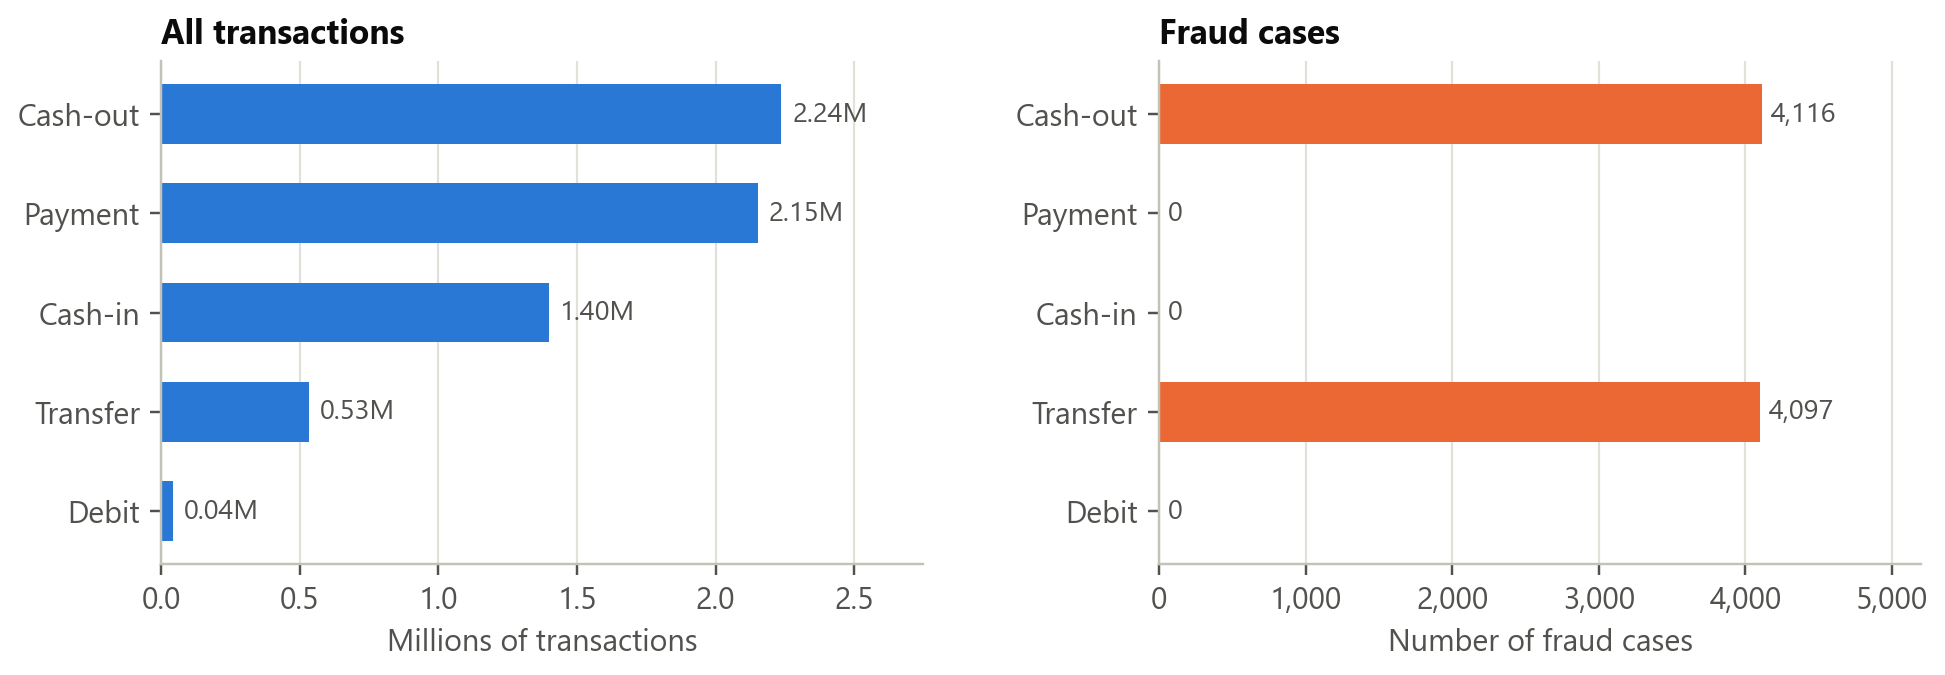
\includegraphics[width=\linewidth]{figures/data_types.png}
\caption{Transactions and fraud cases by payment type}
\label{fig:types}
\end{figure}

\paragraph{Fraud stays steady while normal activity goes up and down.}
Figure~\ref{fig:daily} shows how busy each day was. On most of the first 17 days
there are around 400,000 transactions a day, while later days often have fewer
than 60,000. The number of fraud cases, however, stays between about 220 and 320
every day. The simulator adds fraud at a steady pace no matter how busy the day
is. As a result, fraud is a much larger share of activity on quiet days: on the
very last day, all 272 transactions are fraud. A model must therefore not rely on
how busy a day is.

\begin{figure}[H]
\centering
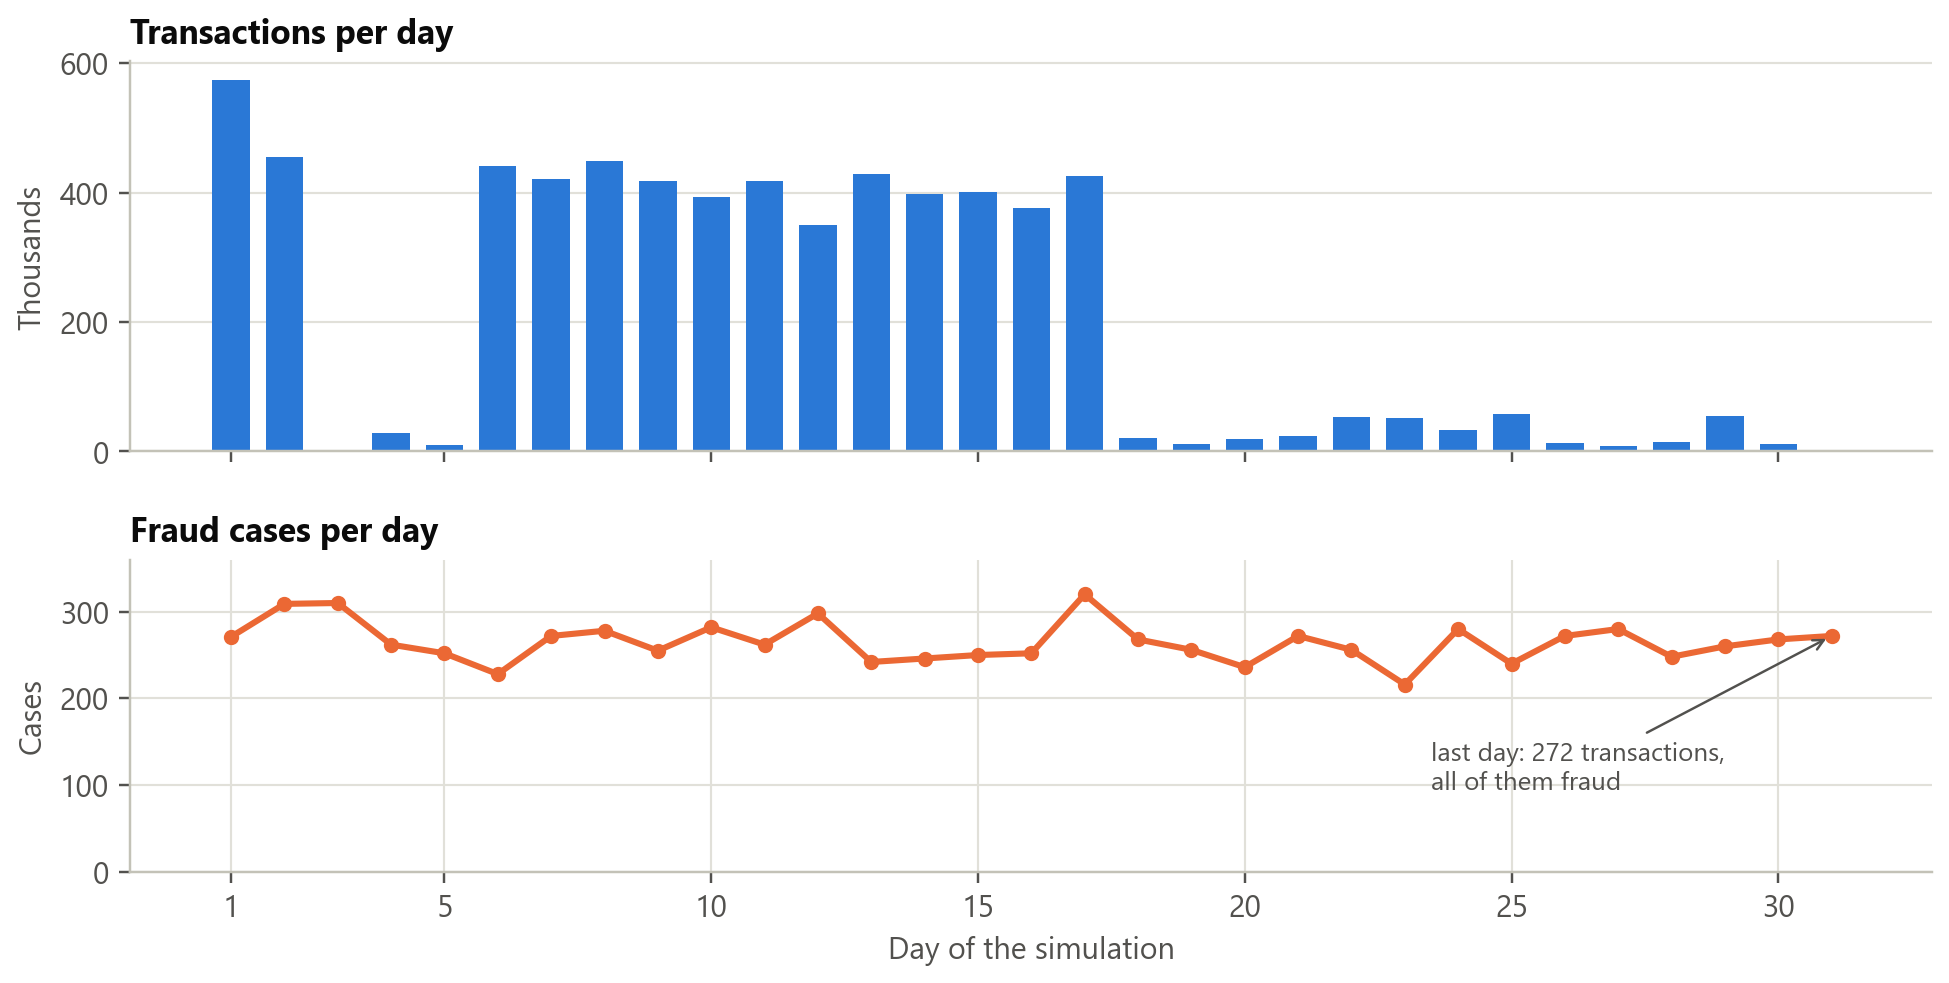
\includegraphics[width=\linewidth]{figures/data_daily.png}
\caption{Transactions per day (top) and fraud cases per day (bottom)}
\label{fig:daily}
\end{figure}

\paragraph{Fraudulent payments are much larger.} As Figure~\ref{fig:amounts}
shows, an average fraudulent transaction moves about 1.47 million units, roughly
eight times more than an average genuine one (about 178,000). In total, fraud
moves more than 12 billion units. This is why even catching a few more fraud
cases matters.

\begin{figure}[H]
\centering
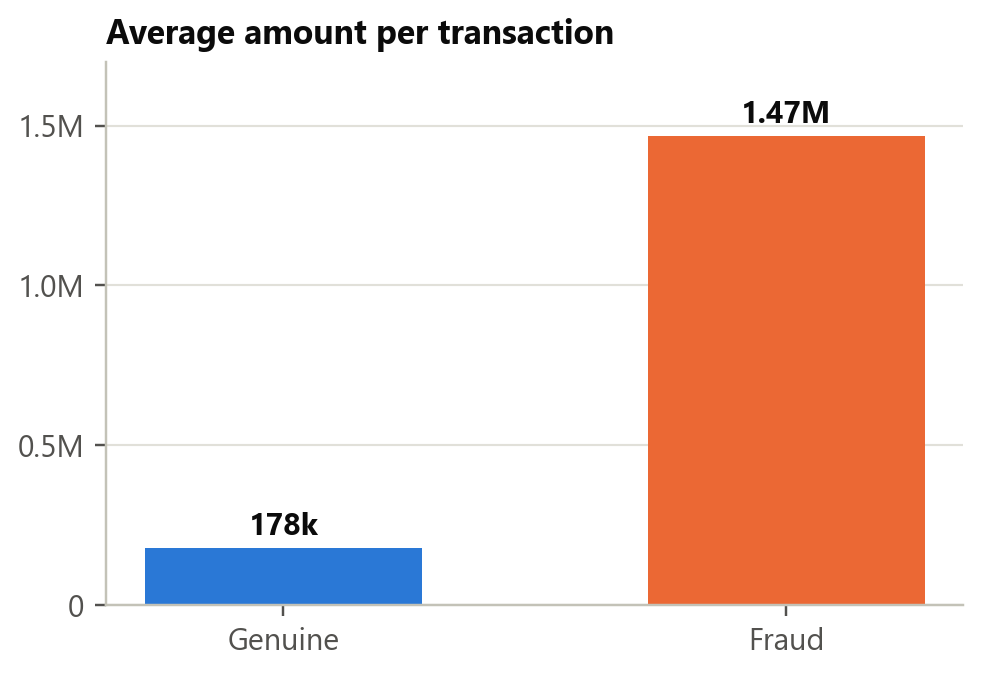
\includegraphics[width=0.55\linewidth]{figures/data_amounts.png}
\caption{Average amount of a genuine and a fraudulent transaction}
\label{fig:amounts}
\end{figure}

Finally, the simulator's own simple rule (flag transfers above 200,000) catches
only 16 of the 8,213 fraud cases. A fixed rule like this is clearly not enough,
which is why we used a trained model.

% ===========================================================================
\section{Literature Review}
% ===========================================================================

\paragraph{ETL and ELT.} In ETL (extract, transform, load), data is cleaned
before it is stored. In ELT (extract, load, transform), the raw data is stored
first and cleaned afterwards. ELT became popular once storage became cheap. Its
main benefit is that the raw copy is always there, so any step can be run again
later \citep{kleppmann2017designing}. The medallion pattern is a layered form of
ELT.

\paragraph{Message logs.} Apache Kafka made the idea of an append-only message
log popular for real-time systems \citep{kreps2011kafka}. Messages with the same
key always go to the same partition, so their order is kept. Stored messages can
be read again later. Many Kafka systems also have a \emph{dead-letter queue}, a
separate topic where bad records are kept so they can be checked later.

\paragraph{Distributed processing.} Apache Spark processes large amounts of data
by splitting the work across many parts. It supports SQL, data frames and
machine learning through its MLlib library \citep{zaharia2016spark}, which makes
it a good fit for both cleaning data and running a model on millions of rows.

\paragraph{Storage.} A lakehouse stores data as open files but manages it like a
database \citep{armbrust2021lakehouse}. Apache Parquet is the usual file format
\citep{parquet}. It stores data by column and compresses it well, so reading
only a few columns is fast.

\paragraph{Scheduling.} Workflow tools describe a pipeline as a chain of tasks
with a schedule and retries. In Apache Airflow the chain is written in Python,
which makes it easy to track and test \citep{airflow}. Retrying a task is only
safe if running it twice gives the same result as running it once
\citep{kleppmann2017designing}.

\paragraph{Fraud detection with rare cases.} When one class is very rare,
accuracy is misleading. Fraud models are judged on \emph{precision} (how many
alerts are real fraud), \emph{recall} (how much of the fraud is caught) and
their balance, the F1 score. \citet{saito2015precision} show that
precision-recall analysis is more useful than ROC curves in this case. The cut-off
score for raising an alert should also be tuned, because it trades missed fraud
against false alarms \citep{dalpozzolo2015calibrating}. Tree-based models such as
random forests \citep{breiman2001random} and gradient-boosted trees
\citep{friedman2001greedy} work well on this kind of table data.

\paragraph{Serving results.} Dashboards and APIs usually read from a regular
database. PostgreSQL can update a row if it already exists instead of adding a
copy \citep{postgres}, which makes loading data again harmless. FastAPI makes it
easy to put that data behind a web API \citep{fastapi}.

% ===========================================================================
\section{Materials and Methods}
% ===========================================================================

\subsection{Tools and Platforms}
Table~\ref{tab:stack} lists the main tools. All of them are free and open
source, and they all run in Docker containers on one machine.

\begin{table}[H]
\centering
\caption{Tools used in the project}
\label{tab:stack}
\begin{tabularx}{\linewidth}{lLl}
\toprule
Purpose & Tool & Version \\
\midrule
Programming & Python & 3.11 \\
Message broker & Apache Kafka, with Kafka UI & Confluent 7.6 \\
Record checks & Pydantic & 2.x \\
Processing and ML & Apache Spark (PySpark, MLlib) & 4.2.0 \\
File format & Apache Parquet & -- \\
Scheduling & Apache Airflow & 2.7.2 \\
Database & PostgreSQL & 15 \\
API and dashboard & FastAPI, HTML and JavaScript & 0.110+ \\
Packaging & Docker, Docker Compose & -- \\
Testing & pytest & 8.x \\
\bottomrule
\end{tabularx}
\end{table}

\subsection{System Architecture}
Figure~\ref{fig:architecture} shows how the parts fit together. A Python program
sends the transactions to Kafka. Spark reads the same file and builds the
Bronze, Silver and Gold layers. A check makes sure the layers are complete before
the model scores the Gold data. The scores are saved in PostgreSQL and shown
through the API and dashboard. Airflow runs all of these steps in order. Each
step is its own script, so each part could be built and tested separately, and
any step can also be run by hand.

\begin{figure}[H]
\centering
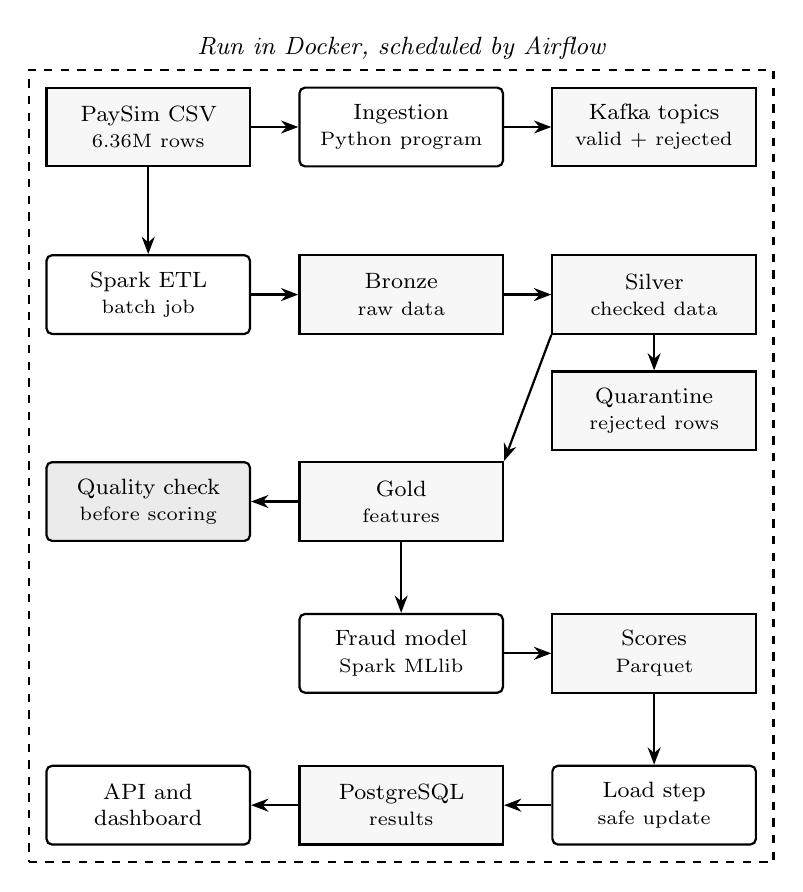
\begin{tikzpicture}[node distance=0.55cm and 0.6cm]
\node[store] (csv) {PaySim CSV\\\scriptsize 6.36M rows};
\node[proc, right=of csv] (ing) {Ingestion\\\scriptsize Python program};
\node[store, right=of ing] (kafka) {Kafka topics\\\scriptsize valid + rejected};

\node[proc, below=1.1cm of csv] (etl) {Spark ETL\\\scriptsize batch job};
\node[store, right=of etl] (bronze) {Bronze\\\scriptsize raw data};
\node[store, right=of bronze] (silver) {Silver\\\scriptsize checked data};
\node[store, below=0.45cm of silver] (quar) {Quarantine\\\scriptsize rejected rows};
\node[store, below=1.6cm of bronze] (gold) {Gold\\\scriptsize features};

\node[tproc, left=of gold] (qc) {Quality check\\\scriptsize before scoring};
\node[proc, below=0.9cm of gold] (ml) {Fraud model\\\scriptsize Spark MLlib};
\node[store, right=of ml] (pred) {Scores\\\scriptsize Parquet};
\node[proc, below=0.9cm of pred] (load) {Load step\\\scriptsize safe update};
\node[store, left=of load] (pg) {PostgreSQL\\\scriptsize results};
\node[proc, left=of pg] (api) {API and\\dashboard};

\draw[arr] (csv) -- (ing);
\draw[arr] (ing) -- (kafka);
\draw[arr] (csv) -- (etl);
\draw[arr] (etl) -- (bronze);
\draw[arr] (bronze) -- (silver);
\draw[arr] (silver) -- (quar);
\draw[arr] (silver.south west) -- (gold.north east);
\draw[arr] (gold) -- (qc);
\draw[arr] (gold) -- (ml);
\draw[arr] (ml) -- (pred);
\draw[arr] (pred) -- (load);
\draw[arr] (load) -- (pg);
\draw[arr] (pg) -- (api);

\node[draw, dashed, thick, inner sep=6pt, fit=(ing)(etl)(qc)(ml)(load)(kafka)(quar)(api),
      label={[font=\small\itshape]above:Run in Docker, scheduled by Airflow}] {};
\end{tikzpicture}
\caption{How the parts of the system connect. Shaded boxes store data; white boxes do work}
\label{fig:architecture}
\end{figure}

\subsection{How the Data Moves}
Different parts of the system use different patterns. When data comes in, the
Python program only checks each record and then passes it to Kafka unchanged.
Inside the lakehouse we follow ELT: Spark first stores the raw records in Bronze
and only then builds Silver and Gold from them. Because the raw copy is kept, we
can change a cleaning rule or a feature later and rebuild the other layers
without reading the original file again. Finally, the model turns the Gold data
into scores, which are copied into PostgreSQL as they are.

\subsection{Bringing Data In with Kafka}
The data file is 494~MB, so the Python program reads it 5,000 rows at a time to
keep memory use low. Each row is checked against a set of rules written with
Pydantic: the columns must have the right type, the payment type must be one of
the five known values, amounts and balances cannot be negative, the fraud label
must be 0 or 1, and account names must look correct.

Good records go to the Kafka topic \code{financial-transactions}. Each message
uses the sender's account as its key, so all payments from one account stay in
order. Records that fail a check go to a second topic,
\code{financial-transactions-dlq}, together with the error and the row number,
so nothing is lost without a trace. Kafka confirms a message only after it is
safely stored, and failed sends are retried three times. The program can also
replay the file slowly to imitate a live stream, or check the file without
sending anything.

\subsection{Cleaning and Preparing Data with Spark}
\paragraph{Bronze.} Spark stores every record exactly as it arrived, in
compressed Parquet files split by hour. It also adds four extra columns: a batch
number, the time it was stored, where it came from, and a unique fingerprint of
the record that helps spot duplicates later.

\paragraph{Silver.} Spark gives each column its correct type and applies seven
rules: the hour must be 1 or more, the payment type must be valid, the amount
must not be missing or negative, both account names must be valid, and none of
the four balances can be missing or negative. Records that break a rule are moved
to a \emph{quarantine} table together with the rule they broke. The remaining
records are checked for duplicates, using the hour, type, amount, both account
names and the sender's balances to decide whether two rows are the same payment.

\paragraph{Gold.} Spark gives every transaction a permanent ID, built from the
same fields used for de-duplication, so the ID stays the same every time the
pipeline runs. It then adds the ten features in Table~\ref{tab:features}, plus
summary tables per customer and per hour. The fraud label is kept only to check
the model; it is never used as an input.

\begin{table}[H]
\centering
\caption{Features added in the Gold layer}
\label{tab:features}
\begin{tabularx}{\linewidth}{lL}
\toprule
Feature & What it means \\
\midrule
\code{orig\_balance\_error} & How far the sender's balance change differs from the amount \\
\code{dest\_balance\_error} & How far the receiver's balance change differs from the amount \\
\code{is\_high\_risk\_type} & 1 for transfers and cash-outs \\
\code{is\_merchant\_dest} & 1 if the money goes to a merchant \\
\code{is\_customer\_dest} & 1 if the money goes to a customer \\
\code{orig\_zero\_balance\_flag} & 1 if the sender had no money before \\
\code{dest\_zero\_balance\_flag} & 1 if the receiver's balance is zero before and after \\
\code{is\_orig\_fully\_emptied} & 1 if the sender's account is emptied \\
\code{amount\_to\_orig\_balance\_ratio} & Amount compared with the sender's starting balance \\
\code{is\_large\_transaction} & 1 if the amount is 200,000 or more \\
\bottomrule
\end{tabularx}
\end{table}

\subsection{The Fraud Detection Model}
For the pipeline, the model is one step: it reads the Gold layer and writes a
score for every transaction. One point needed care. Some columns, such as the
balances \emph{after} the payment, make a model look excellent in testing, but a
bank must decide before the money moves, when those values do not exist yet.
Using them would be \emph{data leakage}. Our model therefore uses only what is
known at the time of the payment: the amount, the starting balances, the payment
type, the hour and the safe flags from Table~\ref{tab:features}.

We split the Gold data into 80\% for training and 20\% for testing, and compared
logistic regression, random forests and gradient-boosted trees. Gradient-boosted
trees did best. The model gives each payment a score between 0 and 1, and an
alert is raised when the score is 0.4 or more, which gave the best balance
between catching fraud and avoiding false alarms. The trained model and its
settings are saved in the project, so every pipeline run uses the same model.

\subsection{Running Everything with Airflow}
One Airflow workflow, \code{fraud\_detection\_pipeline}, runs the whole process
every six hours. It has seven steps, shown in Figure~\ref{fig:dag}. Each step
runs one of the project scripts, so a step in Airflow does exactly what it would
do if we ran it by hand. If a step fails, the steps after it do not start.

\begin{figure}[H]
\centering
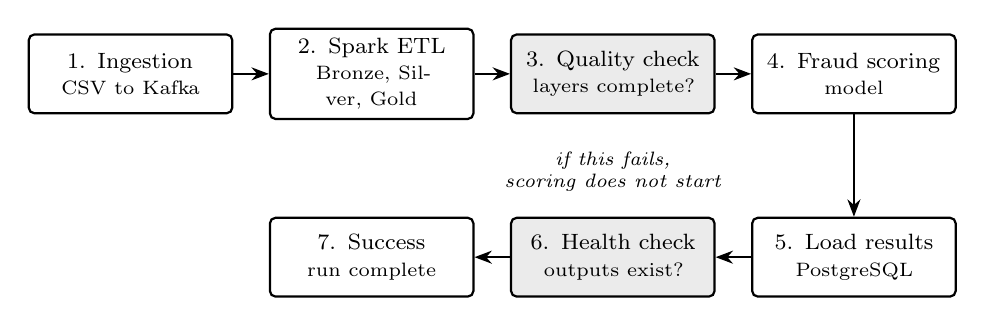
\begin{tikzpicture}[node distance=0.45cm and 0.45cm]
\node[proc] (t1) {1. Ingestion\\\scriptsize CSV to Kafka};
\node[proc, right=of t1] (t2) {2. Spark ETL\\\scriptsize Bronze, Silver, Gold};
\node[tproc, right=of t2] (t3) {3. Quality check\\\scriptsize layers complete?};
\node[proc, right=of t3] (t4) {4. Fraud scoring\\\scriptsize model};
\node[proc, below=1.3cm of t4] (t5) {5. Load results\\\scriptsize PostgreSQL};
\node[tproc, left=of t5] (t6) {6. Health check\\\scriptsize outputs exist?};
\node[proc, left=of t6] (t7) {7. Success\\\scriptsize run complete};
\draw[arr] (t1) -- (t2);
\draw[arr] (t2) -- (t3);
\draw[arr] (t3) -- (t4);
\draw[arr] (t4) -- (t5);
\draw[arr] (t5) -- (t6);
\draw[arr] (t6) -- (t7);
\node[note, below=0.35cm of t3] {if this fails,\\scoring does not start};
\end{tikzpicture}
\caption{The seven steps of the Airflow workflow}
\label{fig:dag}
\end{figure}

A few settings keep the workflow safe. Each failed step is retried up to three
times, five minutes apart, which covers short problems such as Kafka still
starting up. Only one run can happen at a time, so two runs never write to the
same files together. If the workflow is paused for a while, it does not try to
catch up on every missed run; it simply runs once. The quality check in step 3
stops the run if any layer is missing, unreadable or empty, so the model never
scores incomplete data.

\subsection{Serving the Results}
The scores are saved in a PostgreSQL database called \code{fraud}. Each
transaction appears only once, because its permanent ID is the key of the table.
When the results are loaded again, existing rows are updated instead of copied.
The whole load happens in one step: either all the rows are saved or none are,
so a failed load never leaves half the results behind. Every load is also
recorded with its status, row count and time.

A FastAPI service makes the results available on the web. It can check that the
system is running, list the flagged payments from riskiest to least risky, look
up a single transaction, and give overall statistics. If nothing has been loaded
yet, it returns a clear message instead of an error.

The same service shows a dashboard for analysts who do not want to use an API
(Figure~\ref{fig:dashboard}). At the top it shows the steps of the pipeline and
the main numbers: transactions checked, transactions flagged, how much fraud is
caught and how many alerts are real. Below that are a chart of alerts by payment
type and a box to check any single transaction. When a transaction is opened, the
dashboard explains its score in a plain sentence and shows it against the
cut-off. The colours always mean the same thing: black for high risk, yellow for
alerts that need a look, and green for results that are fine.

\begin{figure}[H]
\centering
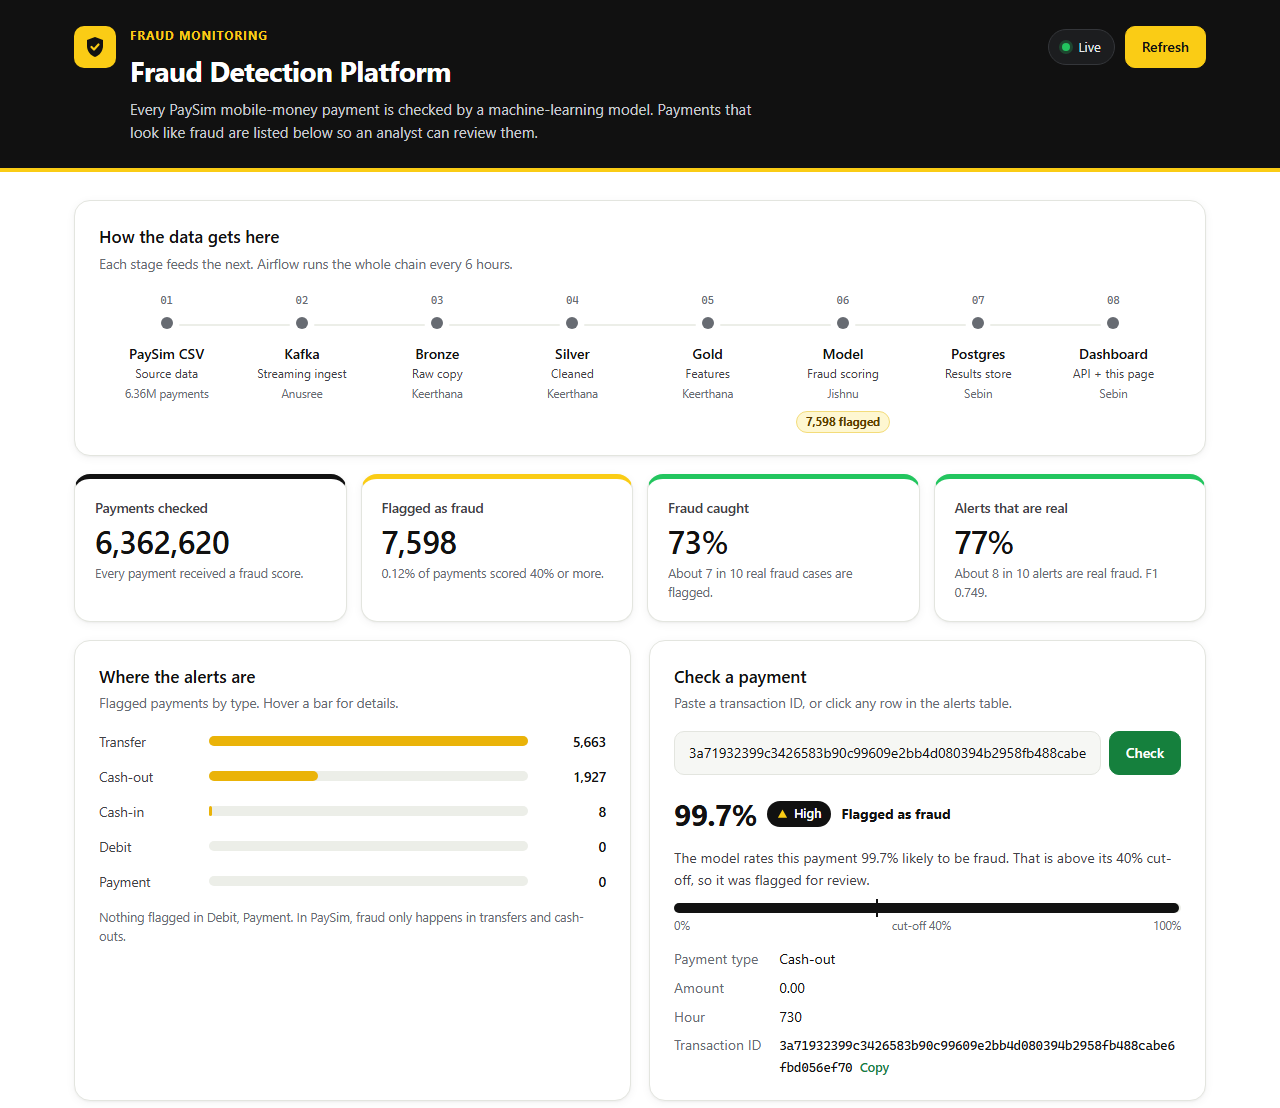
\includegraphics[width=\linewidth]{figures/dashboard_overview.png}
\caption{The analyst dashboard showing the results for the full dataset}
\label{fig:dashboard}
\end{figure}

\subsection{Packaging with Docker}
All the services (Kafka, PostgreSQL, Airflow and the API) are described in one
Docker Compose file and start with a single command. The Airflow container also
includes Java and Spark, so the whole pipeline runs inside it. The project
folders are shared with the containers, so code changes take effect straight
away and the data files stay on the computer. Tool versions are fixed, so the
setup builds the same way on every machine.

% ===========================================================================
\section{Results and Evaluation}
% ===========================================================================

\subsection{Running the Full Pipeline}
We ran the workflow on the full PaySim file. All seven steps succeeded and the
whole run took about 24 minutes on one laptop. Loading all the scores into
PostgreSQL took 3 minutes and 29 seconds, and looking up alerts in the database
takes only milliseconds.

\paragraph{No record was lost or duplicated.} The first thing we checked was
that every record made it through. After the run we counted the rows at every
stage (Figure~\ref{fig:layers}, left). The CSV file, Bronze, Silver, Gold, the
scores and the PostgreSQL table all hold exactly 6,362,620 rows. No row was put
in quarantine, which we expected because the simulated data is clean.

\paragraph{The layers take more space than the original file.} Parquet files are
usually smaller than CSV, but here every layer is larger than the 494~MB input
(Figure~\ref{fig:layers}, right). There are two reasons. First, each layer adds
columns. Bronze adds a batch number, a time stamp, the source file and a
64-character fingerprint of each record; the fingerprint looks random, so it
hardly compresses. Gold adds a permanent ID and ten feature columns, which makes
it the largest layer at 1,260~MB. Second, the data is split into 743 hourly
folders, so the files are small: Silver alone has 2,868 files of about 250~KB
each on average. Many small files compress less well and are slower to read.
This was not a problem at this size, but with more data the files should be
merged into fewer, larger ones.

\begin{figure}[H]
\centering
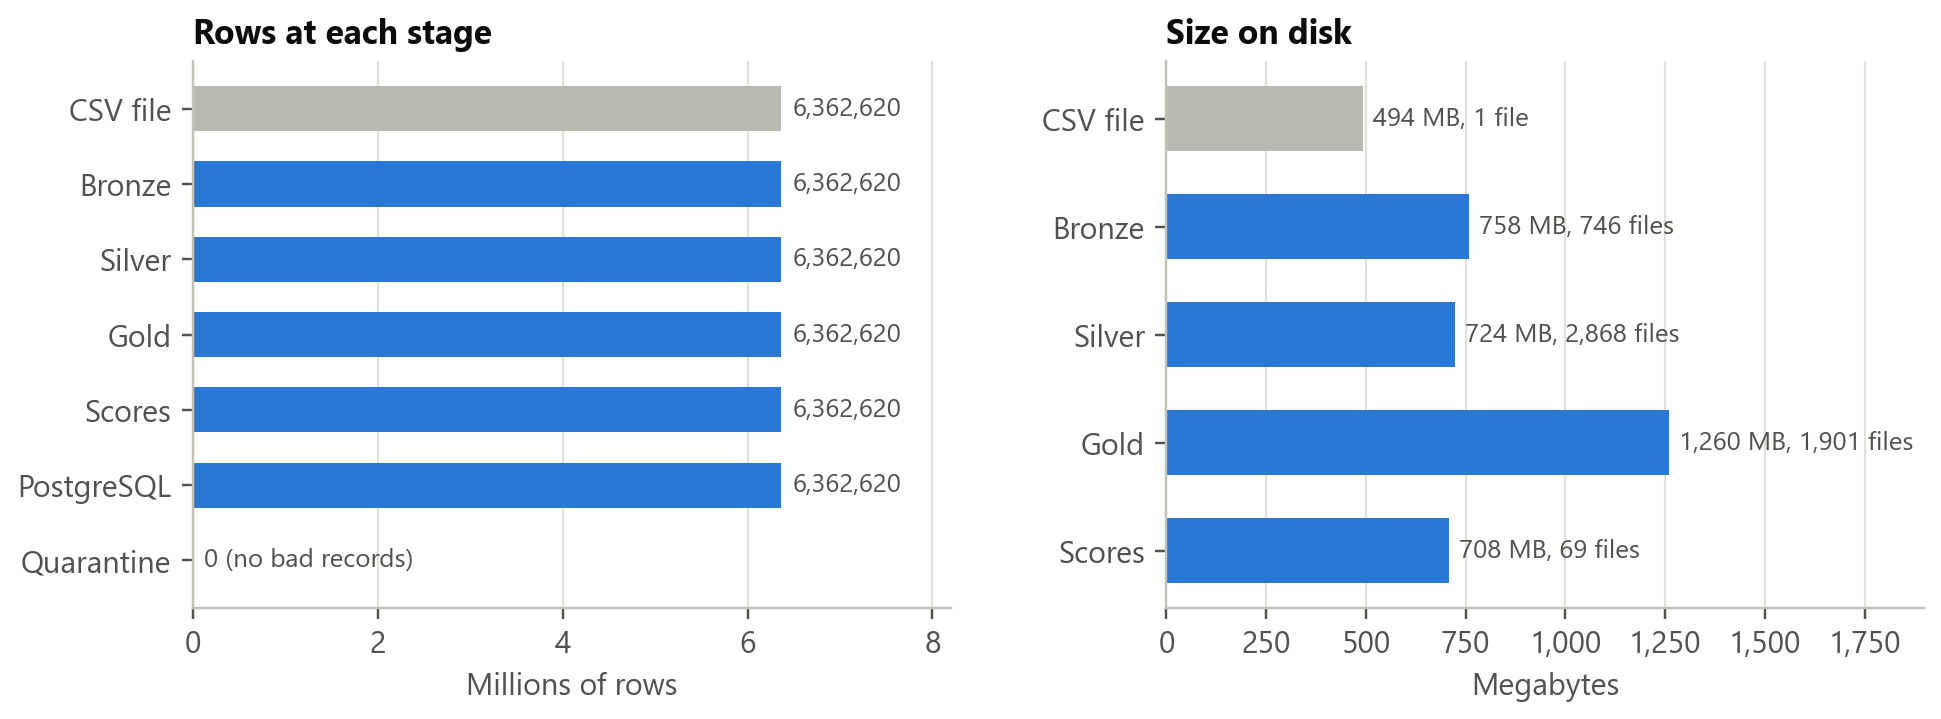
\includegraphics[width=\linewidth]{figures/pipeline_layers.png}
\caption{Rows (left) and storage on disk (right) at each stage, counted after the full run}
\label{fig:layers}
\end{figure}

Getting to this point took several attempts. Most problems appeared only when
all the parts ran together for the first time:
\begin{itemize}
  \item the saved model would not load, because it was made with a newer version
        of Spark than the one installed, so we fixed the Spark version;
  \item the Airflow setup could not install Java the usual way, so we copied it
        from another ready-made image;
  \item two libraries needed different versions of the same package, so we chose
        versions that work together;
  \item the workflow could not find the scripts inside Docker, because it looked
        for them in the wrong folder;
  \item each run added another full copy of the data, so we changed the pipeline
        to replace the old layers instead.
\end{itemize}
Each part worked on its own, but small differences in versions, folders and
settings only showed up once everything was put together.

\subsection{How Well the Model Works}
The model is one step of the pipeline, so we only summarise its results here.
Figure~\ref{fig:confusion} compares its decisions with the true labels over the
whole dataset. It caught 5,938 of the 8,213 fraud cases and raised 1,660 false
alarms among more than 6.3 million genuine payments.

\begin{figure}[H]
\centering
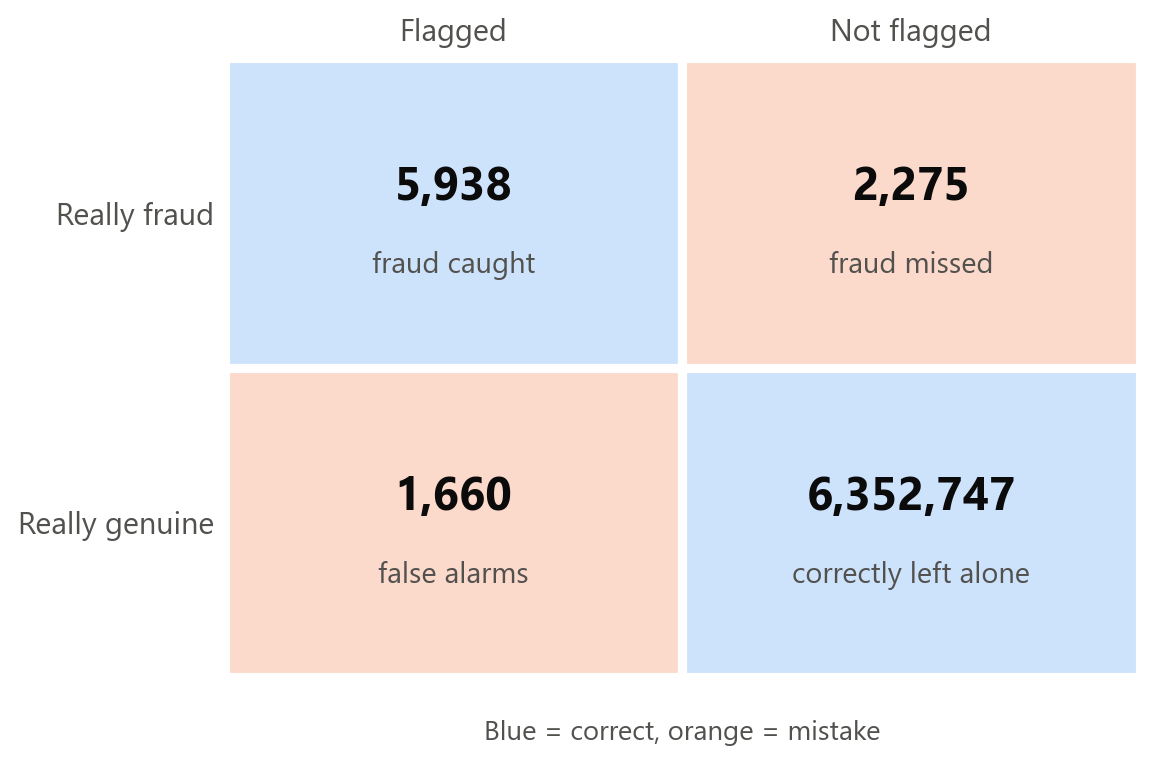
\includegraphics[width=0.7\linewidth]{figures/model_confusion.png}
\caption{Model decisions compared with the true labels (cut-off 0.4)}
\label{fig:confusion}
\end{figure}

On the test data, which the model never saw during training, the precision is
0.773, the recall 0.726 and the F1 score 0.749. In simple terms, about 8 out of
every 10 alerts are real fraud, and about 7 out of every 10 fraud cases are
caught. Over the 31 days the model raised 7,598 alerts, about 245 a day, which a
small team could check.

\paragraph{Why accuracy alone is misleading.} The model's accuracy, the share of
all decisions that are correct, is 99.94\%. That sounds excellent, but a model
that never flags anything would score 99.87\%, because almost every payment is
genuine. Figure~\ref{fig:accuracy} shows the difference that matters: our model
catches 72.3\% of the fraud, while the ``never flag'' model catches none.

\begin{figure}[H]
\centering
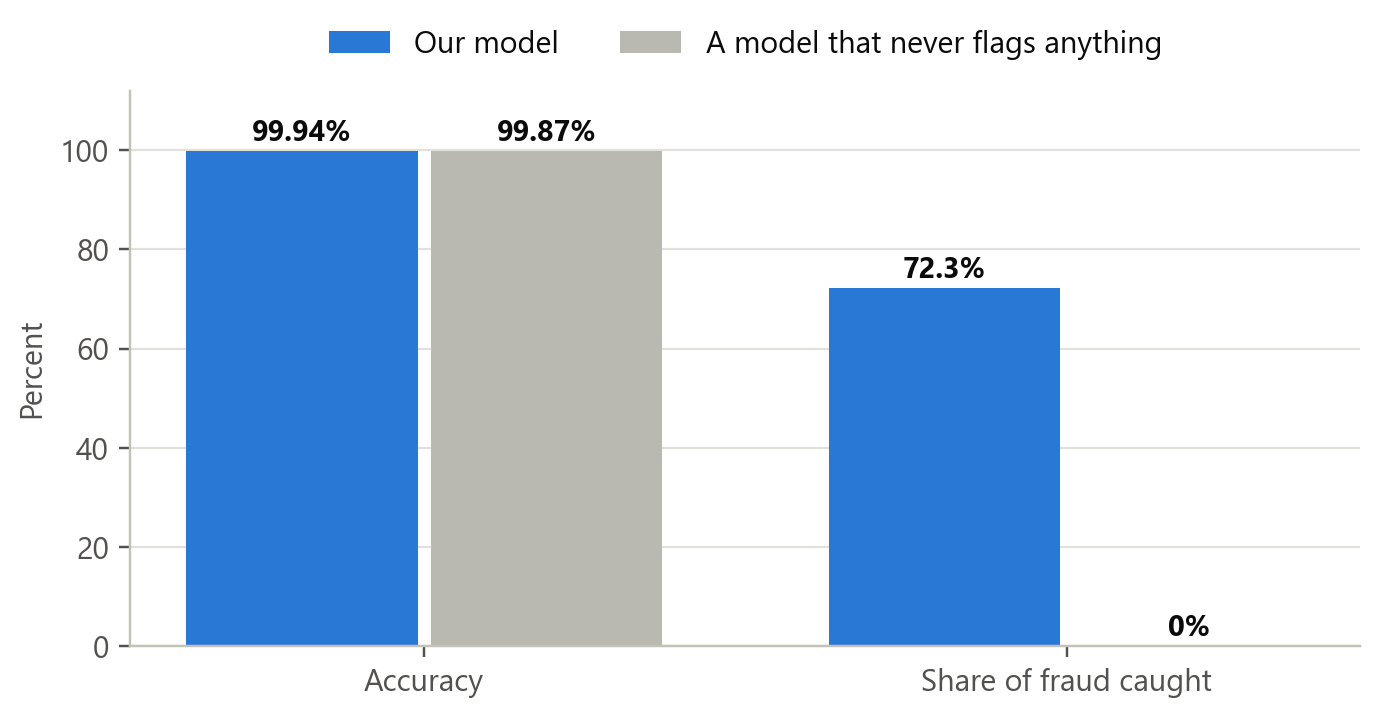
\includegraphics[width=0.75\linewidth]{figures/model_accuracy.png}
\caption{Both models look almost perfectly accurate, but only ours catches fraud}
\label{fig:accuracy}
\end{figure}

\paragraph{What the analyst sees.} Of the 7,598 alerts, 5,663 are transfers,
1,927 are cash-outs and only 8 are cash-ins. Since no cash-in in the data is ever
fraud, those 8 are false alarms that a simple rule could remove.
Figure~\ref{fig:alerts} shows the riskiest alerts in the dashboard. The top ones
are cash-outs of zero. This looks odd, but it is a real pattern: PaySim has 16
zero-amount transactions and every one of them is fraud.

\begin{figure}[H]
\centering
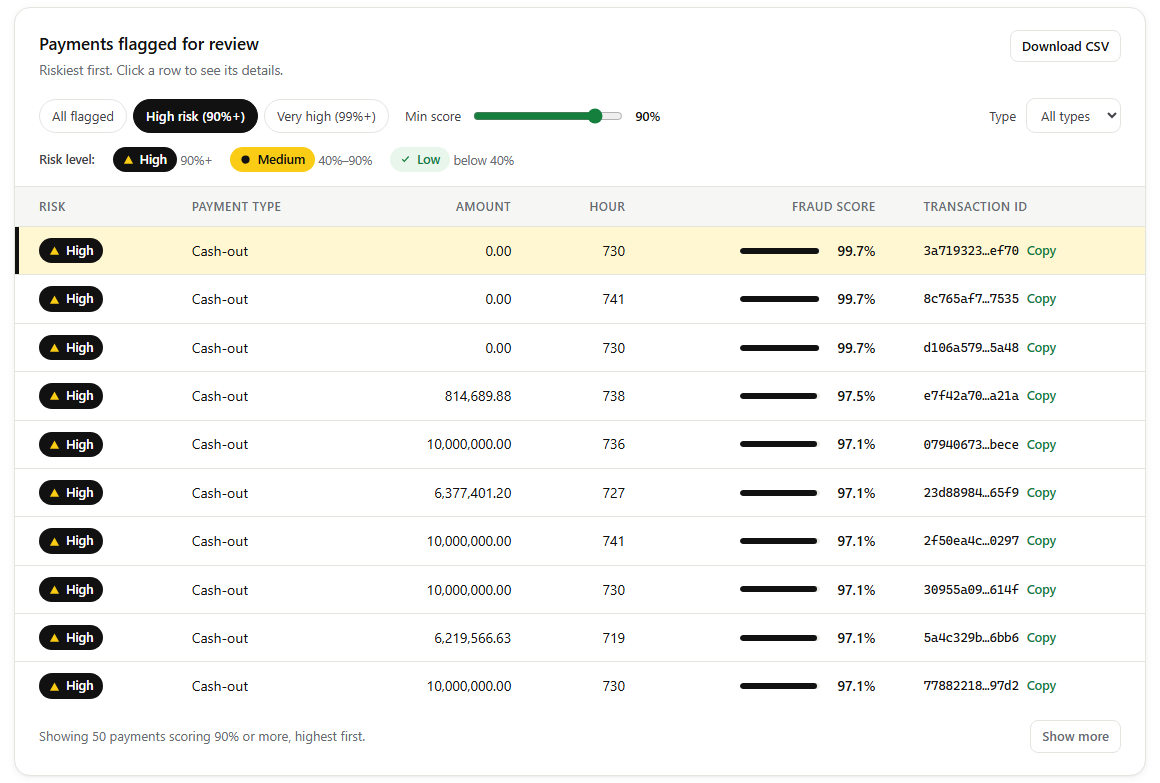
\includegraphics[width=\linewidth]{figures/dashboard_alerts.png}
\caption{The riskiest alerts in the dashboard, with a fraud score of 90\% or more}
\label{fig:alerts}
\end{figure}

\subsection{Data Quality and Testing}
We check data quality at three points: when records arrive, when Silver is
built, and just before the model runs. On the full dataset every check passed.
Because clean data does not really test the rules, we also wrote automated
tests. One test file contains three deliberately bad records (a negative amount,
an unknown payment type and a negative balance), and the tests confirm that
exactly these three are moved to quarantine with the right reason, and that
duplicate rows are reduced to one. In total the project has 50 automated tests
covering record checks, file reading, Kafka sending, the lakehouse layers, the
full ETL, and the database and API. Before using the full dataset, we also ran
the whole workflow on a small 12-row sample to make sure every step worked.

\subsection{Reliability}
A key goal was that running a step twice should never create duplicates. Each
step has its own protection. The layers are replaced on every run instead of
added to. Each transaction has a permanent ID, so the same payment always gets
the same ID. The database updates existing rows instead of adding copies, and a
load either fully succeeds or changes nothing. Bad records are kept, not thrown
away. Because of this, Airflow can safely retry any step, and each transaction
still appears exactly once in the results.

\subsection{Discussion}
Giving each tool one clear job, and connecting them only through agreed data
formats, made the system easier to test and to fix. If one part needs to be
replaced, the others do not need to change. The project still has some
limitations:
\begin{itemize}
  \item \textbf{It is not fully real time.} Data enters through Kafka, but the
        scoring runs in batches every six hours, so alerts are not instant.
  \item \textbf{The quality check is basic.} It checks that each layer exists and
        is not empty. It does not yet compare the number of rows between layers
        (we did this by hand for Figure~\ref{fig:layers}) or check for duplicate
        IDs.
  \item \textbf{There are too many small files.} Splitting the data by hour gives
        thousands of small files, which take more space and are slower to read.
        Merging them into fewer, larger files would help as the data grows.
  \item \textbf{It runs on one machine.} If that machine stops, everything stops.
        A full run also needs about 11~GB of memory for Docker, and laptops with
        less memory struggled.
  \item \textbf{The data is simulated.} Real fraud is messier and changes over
        time, as fraudsters adapt to what the model catches.
  \item \textbf{Some parts are missing for real use}, such as logins for the API
        and e-mail alerts when a run fails.
\end{itemize}

% ===========================================================================
\section{Conclusion}
% ===========================================================================

The project produced a working system that checks, cleans, scores and serves
6.36 million transactions in about 24 minutes on one computer, with Airflow
running every step on a schedule. Kafka brings the data in and keeps bad records
aside. Spark stores the data in clear layers, keeps every original record and
prepares the features, and every one of the 6.36 million records reached the
end of the pipeline exactly once. The fraud model, trained only on fair
information, catches about 7 in 10 fraud cases, and about 8 in 10 of its alerts
are real. The results are saved safely in PostgreSQL and shown through an API
and a dashboard, and the whole system starts with one command.

Exploring the data first turned out to be just as important as building the
pipeline: knowing that fraud only appears in transfers and cash-outs, that it
stays steady from day to day, and that fraudulent payments are much larger helped
explain what the model learns. We also learned that bringing all the parts
together takes real time, because the hardest problems only appeared at that
stage. Next steps include scoring payments the moment they arrive, adding
stronger quality checks such as automatic row counts between layers, merging
small files, retraining the model when the data changes, and moving the system
to the cloud with proper logins.

% ===========================================================================
\begin{thebibliography}{99}

\bibitem[{Airflow}(2023)]{airflow}
Apache Software Foundation (2023). \emph{Apache Airflow 2.7 Documentation}.
\url{https://airflow.apache.org/docs/apache-airflow/2.7.2/}

\bibitem[Akidau et~al.(2015)]{akidau2015dataflow}
Akidau, T., Bradshaw, R., Chambers, C., et al. (2015). The Dataflow model: a
practical approach to balancing correctness, latency, and cost in massive-scale,
unbounded, out-of-order data processing. \emph{Proceedings of the VLDB
Endowment}, 8(12), 1792--1803.

\bibitem[Armbrust et~al.(2021)]{armbrust2021lakehouse}
Armbrust, M., Ghodsi, A., Xin, R., \& Zaharia, M. (2021). Lakehouse: a new
generation of open platforms that unify data warehousing and advanced analytics.
\emph{Proceedings of CIDR 2021}.

\bibitem[Breiman(2001)]{breiman2001random}
Breiman, L. (2001). Random forests. \emph{Machine Learning}, 45(1), 5--32.

\bibitem[Dal~Pozzolo et~al.(2015)]{dalpozzolo2015calibrating}
Dal Pozzolo, A., Caelen, O., Johnson, R. A., \& Bontempi, G. (2015). Calibrating
probability with undersampling for unbalanced classification. \emph{Proceedings
of the IEEE Symposium Series on Computational Intelligence}, 159--166.

\bibitem[{FastAPI}(2024)]{fastapi}
Ram\'{\i}rez, S. (2024). \emph{FastAPI Documentation}.
\url{https://fastapi.tiangolo.com/}

\bibitem[Friedman(2001)]{friedman2001greedy}
Friedman, J. H. (2001). Greedy function approximation: a gradient boosting
machine. \emph{Annals of Statistics}, 29(5), 1189--1232.

\bibitem[Kleppmann(2017)]{kleppmann2017designing}
Kleppmann, M. (2017). \emph{Designing Data-Intensive Applications}. O'Reilly Media.

\bibitem[Kreps(2014)]{kreps2014lambda}
Kreps, J. (2014). Questioning the Lambda architecture. \emph{O'Reilly Radar}.

\bibitem[Kreps et~al.(2011)]{kreps2011kafka}
Kreps, J., Narkhede, N., \& Rao, J. (2011). Kafka: a distributed messaging system
for log processing. \emph{Proceedings of the NetDB Workshop}, Athens.

\bibitem[Lopez-Rojas et~al.(2016)]{lopezrojas2016paysim}
Lopez-Rojas, E. A., Elmir, A., \& Axelsson, S. (2016). PaySim: a financial mobile
money simulator for fraud detection. \emph{Proceedings of the 28th European
Modeling and Simulation Symposium (EMSS)}, Larnaca, 249--255.

\bibitem[Marz and Warren(2015)]{marz2015bigdata}
Marz, N., \& Warren, J. (2015). \emph{Big Data: Principles and Best Practices of
Scalable Real-Time Data Systems}. Manning.

\bibitem[{Parquet}(2024)]{parquet}
Apache Software Foundation (2024). \emph{Apache Parquet Documentation}.
\url{https://parquet.apache.org/docs/}

\bibitem[{PostgreSQL}(2023)]{postgres}
PostgreSQL Global Development Group (2023). \emph{PostgreSQL 15 Documentation:
INSERT}. \url{https://www.postgresql.org/docs/15/sql-insert.html}

\bibitem[Saito and Rehmsmeier(2015)]{saito2015precision}
Saito, T., \& Rehmsmeier, M. (2015). The precision-recall plot is more informative
than the ROC plot when evaluating binary classifiers on imbalanced datasets.
\emph{PLoS ONE}, 10(3), e0118432.

\bibitem[Zaharia et~al.(2016)]{zaharia2016spark}
Zaharia, M., Xin, R. S., Wendell, P., et al. (2016). Apache Spark: a unified
engine for big data processing. \emph{Communications of the ACM}, 59(11), 56--65.

\end{thebibliography}

\end{document}
